
\subsection{Case of set $1$ parameters in table \ref{table:Reference solution, using MC with $500$ time steps, of Call option price under rBergomi model, for different parameter constellation.}}\label{appendix:Case of set 1 parameters}
%\subsubsection*{Without Richardson extrapolation}
%\begin{table}[!h]
%	\centering
%	\begin{tabular}{l*{6}{c}r}
%		Method \textbackslash  Steps            & $2$ & $4$ & $8$  \\
%		\hline
%%		MISC ($\text{TOL}_{\text{MISC}}=5.10^{-1}$)  & $0.1097$ & $0.0926$ & $0.0807$  \\
%		MISC ($\text{TOL}_{\text{MISC}}=10^{-1}$)  &$0.1097$ & $0.0926$ & $0.0791$   \\
%%		MISC ($\text{TOL}_{\text{MISC}}=5.10^{-2}$)  & $0.1097$ & $0.0890$ & $0.0849$  \\
%		MISC ($\text{TOL}_{\text{MISC}}=10^{-2}$)  & $0.1119$&  $0.1023$ & $0.0910$  \\
%		MISC ($\text{TOL}_{\text{MISC}}=10^{-3}$)        & $0.1195$ &$0.1023$ &   $0.0910$  \\
%		MISC ($\text{TOL}_{\text{MISC}}=10^{-4}$)        & $0.1218$ &$0.1023$ &  $-$  \\
%		\hline
%		MC method ($M=8.10^{6}$)   & $0.1218 $  & $0.1024 $  & $0.0914$  \\		
%		\hline
%	\end{tabular}
%	\caption{ Call option price of the different methods for different number of time steps. Case of set $2$ parameters in table \ref{table:Reference solution, using MC with $500$ time steps, of Call option price under rBergomi model, for different parameter constellation.}, without Richardson extrapolation.}
%	\label{table: Call option price of the different methods for different number of time steps. Case set 2_linear}
%\end{table}

%We show through table \ref{Bias and Statistical errors of MC ($M=10^6$)  for computing Call option price  for different number of time steps. Case set $2$ parameters, without Richardson extrapolation. The numbers between parentheses are the corresponding absolute errors.} the bias and  the statistical error for MC method, related to Section \ref{sec:Weak error plots_no_change}. 
%\FloatBarrier
%\begin{table}[!h]
%	\centering
%	\begin{tabular}{l*{6}{c}r}
%		Method \textbackslash  Steps            & $2$ & $4$ & $8$   \\
%		\hline
%		MC Bias ($M=8.10^6$)   & $0.54
%		$  & $0.29$  & $0.15$   \\	
%		
%		MC Statistical error ($M=8.10^6$)  & $2.5e-03$  & $1.3e-03$  & $6.3e-04$  \\	
%	
%		\hline
%	\end{tabular}
%	\caption{Relative bias and statistical errors of MC, without Richardson extrapolation,  for computing call option price  for different number of time steps}
%	\label{Bias and Statistical errors of MC ($M=10^6$)  for computing Call option price  for different number of time steps. Case set $2$ parameters, without Richardson extrapolation. The numbers between parentheses are the corresponding absolute errors.}
%\end{table}




%In figure \ref{fig:Quadrature_error_set2_linear}, we plot the behavior of  the relative quadrature error with respect to $\text{TOL}_{\text{MISC}}$. The quadrature error (see \eqref{eq:quadrature error}) is computed by subtracting the MISC solution from the biased solution, computed with sufficiently large  number of samples.




%\begin{figure}[h!]
%	\centering
%	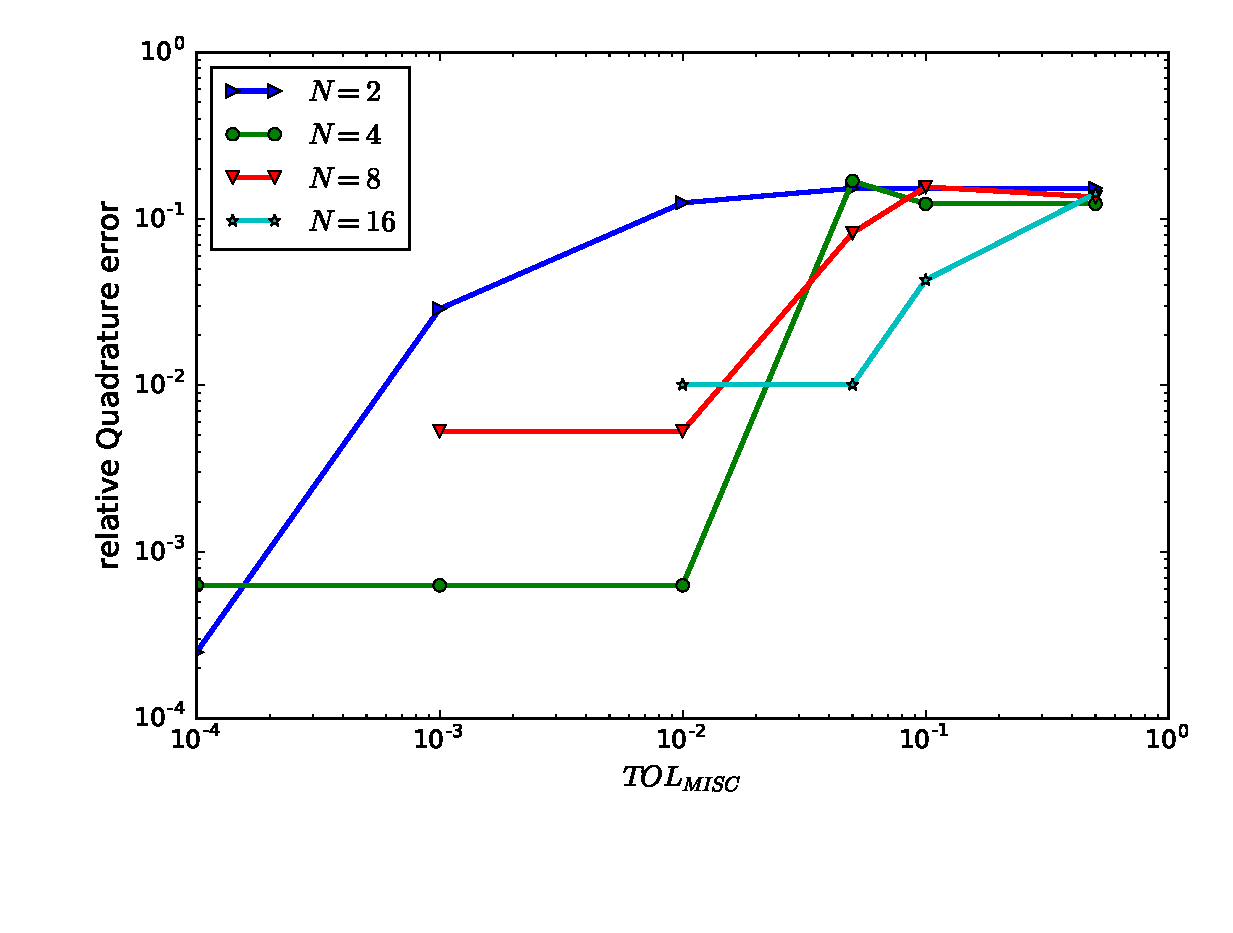
\includegraphics[width=0.4\linewidth]{./figures/rBergomi_MISC_quadratre_error/vs_TOL/set2/relative_quad_error_wrt_MISC_TOL_set2_non_rich_linear}
%	
%	
%	\caption{Quadrature error of MISC, without Richardson extrapolation, with different tolerances, to compute call option price for different number of time steps.}
%%	 See detailed values  in table \ref{Quadrature error of MISC to compute Call option price of the different tolerances for different number of time steps. Case  set $2$ parameters, without Richardson extrapolation. The numbers between parentheses are the corresponding absolute errors,linear}.}
%	\label{fig:Quadrature_error_set2_linear}
%\end{figure}




%
%\FloatBarrier
%
%\begin{table}[h!]
%	\centering
%	\begin{tabular}{l*{6}{c}r}
%	\toprule[1.5pt]
%	Method & & Steps  & &     \\
%	\hline
%		    & $2$ & $4$ & $8$  & $16$  \\
%		\hline
%
%		ASGQ ($\text{TOL}_{\text{ASGQ}}=10^{-1}$)  & $\underset{(0.54,0.15)}{\mathbf{
%			0.69}}$& $ \underset{(0.29,0.13)}{\mathbf{    
%			0.42}}$ & $ \underset{(0.15,0.16)}{\mathbf{     
%			0.31
%		}}$   & $ \underset{(0.07,0.04)}{\mathbf{     
%			0.11
%		}}$ \\
%
%		ASGQ ($\text{TOL}_{\text{ASGQ}}=10^{-2}$)  & $\underset{(0.54,0.12)}{\mathbf{ 
%			0.66}}$ & $ \underset{(0.29,6e-04)}{\mathbf{  0.29}}$ & $\underset{(0.15,0.01)}{\mathbf{    0.16}}$&  $ \underset{(0.07,0.01)}{\mathbf{0.08}}$  \\
%%		MISC ($\text{TOL}_{\text{MISC}}=10^{-3}$)        & $\underset{(0.54,0.10)}{\mathbf{
%%			0.64}}$  &  $ \underset{(0.29,6e-04)}{\mathbf{
%%			0.29
%%		}}$ &  $\underset{(0.15,0.01)}{\mathbf{    \red{0.16}}}$ &  $-$ \\
%%		MISC ($\text{TOL}_{\text{MISC}}=10^{-4}$)        & $\underset{(0.54,3e-04)}{\mathbf{       0.54}}$  & $ \underset{(0.29,6e-04)}{\mathbf{
%%			0.29
%%		}}$  &  $-$ &  $-$\\
%		%\hline
%%		MC    & $\underset{(0.54,3e-03)}{\mathbf{0.54}}$  & $\underset{(0.29,1e-03)}{\mathbf{0.29}}$  &$\underset{(0.15,0.01)}{
%%				\mathbf{0.16}}$ & \\	
%%		M(\# MC samples)   & $8 \times 10^6$  & $8 \times 10^6$  &$10^5$ & \\	
%\hline
%				QMC+smooth    & $\underset{(0.54,0.66)}{\mathbf{1.2}}$  & $\underset{(0.295,0.39)}{\mathbf{0.665 }}$  &$\underset{(0.155,0.19)}{
%				\mathbf{0.345}}$& $\underset{(0.07,0.10)}{
%				\mathbf{0.17}}$ \\	
%		M(\# QMC samples)   & $2^3 \times 2^5= 256$  & $2^3 \times 2^6= 512$  &$2^3 \times 2^7= 1024$  & $2^3 \times 2^8=2048 $ \\
%				\hline
%				MC    & $\underset{(0.54,0.51)}{\mathbf{1.05}}$  & $\underset{(0.295,0.295)}{\mathbf{0.59}}$  &$\underset{(0.155,0.155)}{
%				\mathbf{0.31}}$& $\underset{(0.07,0.07)}{
%				\mathbf{0.14}}$ \\	
%		M(\# MC samples)   & $8 \times 10$  & $16 \times 10$  &$4 \times 10^2$  & $16 \times 10^2$ \\
%		\bottomrule[1.25pt]
%	\end{tabular}
%	\caption{\red{Total relative error of the different methods, without Richardson extrapolation,  to compute the call option prices for different numbers of time steps}. The values between parentheses correspond to the different errors contributing to the total relative error: for ASGQ we report the bias and quadrature errors and for MC and QMC we report the bias and the statistical errors estimates. The number of MC and QMC samples, $M$, are chosen to satisfy \eqref{optimal_number_samples}. \red{We compare two versions of QMC: one that is applied to the non smooth payoff and a second that is applied to the smoothed payoff}. }
%	\label{Total error of MISC and MC to compute Call option price of the different tolerances for different number of time steps. Case $K=1$, $H=0.07$, without Richardson extrapolation. The numbers between parentheses are the corresponding absolute errors,linear}
%\end{table}
%\FloatBarrier
%
%
%
%
%\begin{table}[htbp]
%	\centering
%	\begin{tabular}{l*{6}{c}r}
%		\toprule[1.5pt]
%	Method & & Steps  & &     \\
%	\hline
%	        & $2$ & $4$ & $8$  &$16$  \\
%		\hline
%%		MISC ($\text{TOL}_{\text{MISC}}=5.10^{-1}$)  & $0.08$ & $0.13$ & $0.2$ \\
%		ASGQ ($\text{TOL}_{\text{ASGQ}}=10^{-1}$)  & $0.08$ & $0.13$ & $0.7$  & $163$ \\
%%		ASGQ ($\text{TOL}_{\text{MISC}}=5.10^{-2}$)  & $0.08$ & $0.25$ & $7$   \\
%		ASGQ ($\text{TOL}_{\text{ASGQ}}=10^{-2}$)  & $0.2$& $5$ & $333$ &  $1602$\\
%%		MISC ($\text{TOL}_{\text{MISC}}=10^{-3}$)  &  $2$ & $73$ & $3650$ &  $-$ \\		
%%		MISC ($\text{TOL}_{\text{MISC}}=10^{-4}$)  & $43$ & $1240$ & $-$ &   $-$\\	
%%	
%%		\hline
%%		MC method & $220$  & $358$  & $9$ & \\
%	\hline	
%		QMC method & $0.022$  & $0.045$  & $0.1$ & $0.26$ \\
%		\hline	
%		MC method & $0.004$  & $0.012$  & $0.08$ & $0.8$ \\
%		\bottomrule[1.25pt]	
%%		Ratio of CPU time  $\left(\text{MC}/ \text{MISC} \right)$  &$\red{5}$ & $\red{   72 
%%		}$  & $\red {  0.03	}$   \\
%%		\hline
%	\end{tabular}
%	\caption{Comparison of the computational time (in seconds) of  the different methods, to compute the call option price of the rBergomi model for different numbers of time steps. The average MC CPU time is computed over $100$ runs.}
%	\label{Comparsion of the computational time of  MC and MISC, used to compute Call option price of rBergomi model for different number of time steps. Case $K=1, H=0.07$, linear}
%\end{table}
%\FloatBarrier
%\subsubsection*{With Richardson extrapolation (level $1$)}

%\begin{table}[!h]
%	\centering
%	\begin{tabular}{l*{6}{c}r}
%		Method \textbackslash  Steps    &$1-2$         & $2-4$ & $4-8$ \\
%		\hline
%%		MISC ($\text{TOL}_{\text{MISC}}=5.10^{-1}$)  &$0.1260$ & $0.0756$ & $0.0687$\\
%		MISC ($\text{TOL}_{\text{MISC}}=10^{-1}$)  &$0.1260$ & $0.0756$ & $0.0702$   \\
%		MISC ($\text{TOL}_{\text{MISC}}=5.10^{-2}$)   &$0.1260$ & $0.0716$ & $0.0796$    \\
%		MISC ($\text{TOL}_{\text{MISC}}=10^{-2}$)  &$0.1456$ & $0.0838$ & $0.0796$  \\	
%		MISC ($\text{TOL}_{\text{MISC}}=10^{-3}$)  &$0.1497$ & $0.0838$ & $-$ \\
%		
%%		MISC ($\text{TOL}_{\text{MISC}}=10^{-4}$)  &$0.1501$ & $-$ & $-$ \\
%		\hline
%		MC method ($M=10^{6}$)   & $0.1552 $  & $0.0846 $  & $0.0804$  \\		
%		\hline
%	\end{tabular}
%	\caption{Call option price of the different methods for different number of time steps. Case set $2$ parameters of table \ref{table:Reference solution, using MC with $500$ time steps, of Call option price under rBergomi model, for different parameter constellation.}, using Richardson extrapolation (level $1$)}
%	\label{table:  Call option price of the different methods for different number of time steps. Case set $2$ parameter, using Richardson extrapolation (level $1$),linear}
%\end{table}

%\FloatBarrier
%
%\begin{table}[h!]
%	\centering
%	\begin{tabular}{l*{6}{c}r}
%		Method \textbackslash  Steps            & $1-2$ & $2-4$ & $4-8$  \\
%		\hline
%		MC Bias ($M=10^6$)  &$0.96$  & $0.07$  & $0.015$   \\	
%		
%		MC Statistical error ($M=10^6$)   & $1.3e-02$  & $4.1e-03$  & $2.1e-03$  \\	
%		\hline
%	\end{tabular}
%	\caption{Relative bias and statistical errors of MC, with Richardson extrapolation (level $1$), for computing call option price  for different number of time steps. The numbers between parentheses are the corresponding absolute errors.}
%	\label{Bias and Statistical errors of MC ($M=10^6$)  for computing Call option price  for different number of time steps. Case set $2$ parameters, with Richardson extrapolation (level1). The numbers between parentheses are the corresponding absolute errors.}
%\end{table}
%
%
%\FloatBarrier
%
%
%
%
%
%\begin{figure}[h!]
%	\centering
%	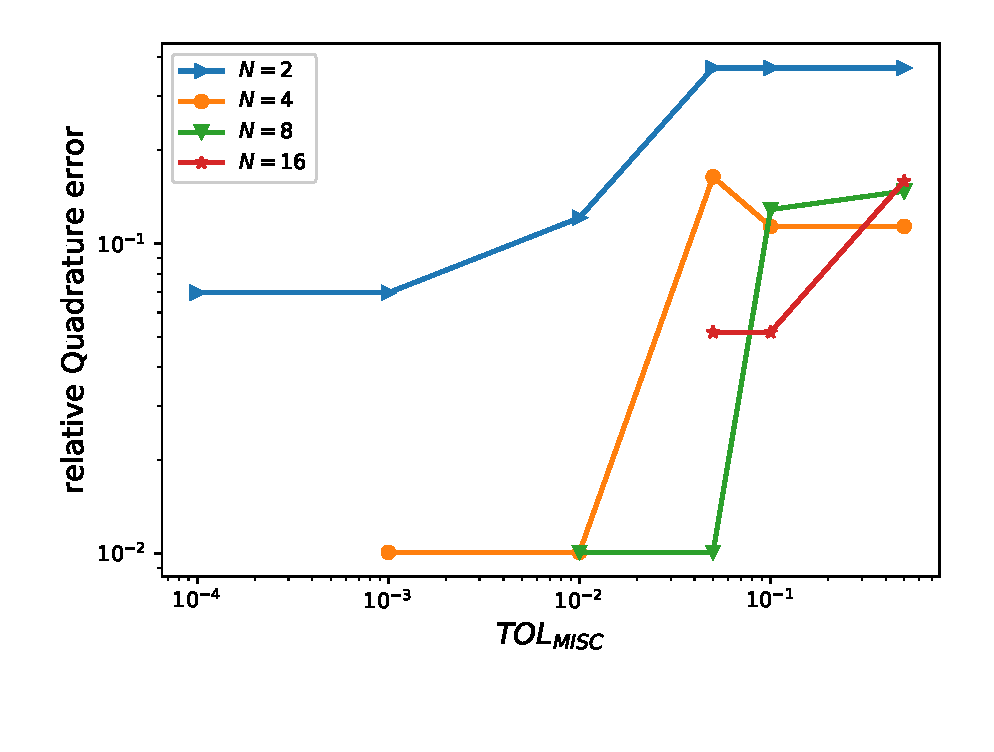
\includegraphics[width=0.4\linewidth]{./figures/rBergomi_MISC_quadratre_error/vs_TOL/set2/relative_quad_error_wrt_MISC_TOL_set2_with_rich_linear}
%	
%	
%	\caption{Quadrature error of MISC,with Richardson extrapolation (level $1$), with different tolerances,  to compute call option price for different number of time steps.}

%	  See detailed values  in table \ref{Quadrature error of MISC to compute Call option price of the different tolerances for different number of time steps. Case set $2$ parameters, with Richardson extrapolation(level $1$). The numbers between parentheses are the corresponding absolute errors,linear}.}
%	\label{fig:Quadrature_error_set2_linear_rich}
%\end{figure}


\begin{table}[h!]
	\begin{small}
		\centering
		\begin{tabular}{l*{6}{c}r}
			\toprule[1.5pt]
			Method & & Steps  & &     \\
			\hline
			& $1-2$ & $2-4$ & $4-8$   & $8-16$  \\
			\hline	
			QMC + level $1$ of  Richardson extrapolation &$\underset{(0.96,0.91)}{\mathbf{1.87}}$  & $\underset{(0.07,0.09)}{\mathbf{0.16}}$ & $\underset{(0.015,0.018)}{\mathbf{0.033}}$ & $\underset{(0.002,0.002)}{\mathbf{0.0044}}$  \\
			M(\# QMC samples) & $128$  & $8192$ & $
			131072$ & $
			2097152$ \\
			\hline
			
			MC + level $1$ of  Richardson extrapolation &$\underset{(0.96,0.92)}{\mathbf{1.88}}$  & $\underset{(0.07,0.07)}{\mathbf{0.14}}$ & $\underset{(0.015,0.015)}{\mathbf{0.03}}$  & $\underset{(0.002,0.0024)}{\mathbf{0.0044}}$\\
			M(\# MC samples) & $4 \times 10$  & $8 \times 10^3$ & $16 \times 10^4$ & $5 \times 10^5$  \\
			\bottomrule[1.25pt]
		\end{tabular}
		\caption{Total relative error of MC and randomized QMC coupled with Richardson extrapolation (level $1$), to compute the call option price  for different numbers of time steps. The values between parentheses correspond to the different errors contributing to the total relative error: the bias and the statistical errors. The number of MC and QMC samples, $M$, are chosen to satisfy \eqref{optimal_number_samples}.}
		\label{Total  error of MISC and MC to compute Call option price of the different tolerances for different number of time steps. Case set $2$ parameters, with Richardson extrapolation(level $1$). The numbers between parentheses are the corresponding absolute errors,relative}
	\end{small}
\end{table}
\FloatBarrier


\begin{table}[h!]
	\centering
	\begin{tabular}{l*{6}{c}r}
		\toprule[1.5pt]
		Method & &   & Steps & &     \\
		\hline
		& $1-2$ & $2-4$ & $4-8$ & $8-16$   \\
		\hline	
		QMC + level $1$ of  Richardson extrapolation  &$0.018$ & $2$  & $18$  & $333$   \\
		\hline	
		MC + level $1$ of  Richardson extrapolation &$
		0.0012$ & $12$  & $152$  & $4400$ \\
		\bottomrule[1.25pt]
	\end{tabular}
	\caption{Comparison of the computational time (in seconds) of  MC and randomized QMC coupled with Richardson extrapolation (level $1$) to compute the call option price of the rBergomi model for different numbers of time steps. The average MC CPU time is computed over $100$ runs.}
	\label{Comparsion of the computational time of  MC and MISC, using Richardson extrapolation (level $1$), used to compute Call option price of rBergomi model for different number of time steps. Case set $2$ parameters,linear}
\end{table}

\FloatBarrier
%	\subsubsection*{With Richardson extrapolation (level $2$)}

%
%		\begin{table}[h!]
%		\centering
%		\begin{tabular}{l*{6}{c}r}
%		Method \textbackslash  Steps           &$1-2-4$ & $2-4-8$ \\
%		\hline
%%		MISC ($\text{TOL}_{\text{MISC}}=5.10^{-1}$)& $0.0587$  & $0.0664 $ \\
%		
%		MISC ($\text{TOL}_{\text{MISC}}=10^{-1}$)  &$0.0587$  &$ 0.0702$   \\
%		MISC ($\text{TOL}_{\text{MISC}}=5.10^{-2}$)  & $0.0401$ & $0.0790$  \\
%		MISC ($\text{TOL}_{\text{MISC}}=10^{-2}$)  & $0.0623$ &  $0.0784$   \\
%%		MISC ($\text{TOL}_{\text{MISC}}=5.10^{-3}$)  & $0.0623$ & $-$   \\
%%		MISC ($\text{TOL}_{\text{MISC}}=10^{-3}$)  & $0.0608$ & $$  \\
%		
%		\hline
%		MC ($M=3.10^6$)  & $ 0.0601$ & $ 0.0787$   \\
%		\hline 
%	\end{tabular}
%	\caption{ Call option price of the different methods for different number of time steps. Case set $2$ parameters in tabel \ref{table:Reference solution, using MC with $500$ time steps, of Call option price under rBergomi model, for different parameter constellation.}, using Richardson extrapolation (level 2).}
%	\label{table: Call option price of the different methods for different number of time steps. Case $K=1,H=0.07$, using Richardson extrapolation_level2,linear}
%\end{table}




%\begin{table}[h!]
%	\centering
%	\begin{tabular}{l*{6}{c}r}
%		Method \textbackslash  Steps            & $1-2-4$ & $2-4-8$  \\
%		\hline
%		MC  Bias  ($M=3.10^6$)   &$ 0.24$  & $ 0.0058$   \\	
%		
%		MC Statistical error ($M=3.10^6$)   & $3.5e-03$  & $  1.8e-03$  \\	
%		
%		
%		
%		\hline
%	\end{tabular}
%	\caption{Relative bias and statistical errors of MC,  with Richardson extrapolation (level $2$), for computing call option price  for different number of time steps. The numbers between parentheses are the corresponding absolute errors.}
%	\label{Bias and Statistical errors of MC ($M=3.10^6$)  for computing Call option price  for different number of time steps. Case set $2$ parameters, with Richardson extrapolation (level2). The numbers between parentheses are the corresponding absolute errors.}
%\end{table}





\begin{table}[!h]
	\begin{small}
		\centering
		\begin{tabular}{l*{6}{c}r}
			\toprule[1.5pt]
			Method & & Steps  & &     \\
			\hline
			& $1-2-4$ & $2-4-8$  \\
			\hline
			
			ASGQ + level $2$ of  Richardson extrapolation ($\text{TOL}_{\text{ASGQ}}=10^{-1}$)  & $\underset{(0.24,0.30)}{\mathbf{ 0.54
			}}$ & $\underset{(0.006,0.107)}{\mathbf{ 0.113}}$ \\
			ASGQ + level $2$ of  Richardson extrapolation ($\text{TOL}_{\text{ASGQ}}=5.10^{-2}$)  & $\underset{(0.24,0.25)}{\mathbf{   0.49
			}}$ & $\underset{(0.006,0.003)}{\mathbf{ 0.009} }$  \\
%			ASGQ + level $2$ of  Richardson extrapolation ($\text{TOL}_{\text{ASGQ}}=10^{-2}$)  & $\underset{(0.24,0.03)}{\mathbf{ 0.27}}$ & $\underset{(0.006,0.003)}{\mathbf{ 0.009 }}$    \\	
			\bottomrule[1.25pt]
		\end{tabular}
		\caption{Total relative error of ASGQ, coupled with Richardson extrapolation (level $2$), to compute the call option price for different numbers of time steps.  The values between parentheses correspond to the different errors contributing to the total relative error: the bias and quadrature errors.}
		\label{Total  error of MISC and MC to compute Call option price of the different tolerances for different number of time steps. Case set $2$ parameters, with Richardson extrapolation(level $2$). The numbers between parentheses are the corresponding absolute errors,linear}
	\end{small}
\end{table}
\FloatBarrier

\begin{table}[!h]
	\centering
	\begin{tabular}{l*{6}{c}r}
		\toprule[1.5pt]
		Method & & Steps  & &     \\
		\hline
		& $1-2-4$ & $2-4-8$   \\
		\hline
		
		ASGQ + level $2$ of  Richardson extrapolation ($\text{TOL}_{\text{ASGQ}}=10^{-1}$)  & $0.2$ & $2$ &   \\
		ASGQ + level $2$ of  Richardson extrapolation ($\text{TOL}_{\text{ASGQ}}=5.10^{-2}$)  & $0.5$ & $74$  \\
%		ASGQ  + level $2$ of  Richardson extrapolation ($\text{TOL}_{\text{ASGQ}}=10^{-2}$)  & $9$ & $3455$   \\
		\bottomrule[1.25pt]
	\end{tabular}
	\caption{Comparison of the computational time (in seconds) of ASGQ coupled with Richardson extrapolation (level $2$) to compute the call option price of the rBergomi model for different numbers of time steps.}
	\label{Comparsion of the computational time of  MC and MISC, using Richardson extrapolation (level $2$), used to compute Call option price of rBergomi model for different number of time steps. Case set $2$ parameters,linear}
\end{table}
\FloatBarrier


\subsection{Case of set $2$ parameters in table \ref{table:Reference solution, using MC with $500$ time steps, of Call option price under rBergomi model, for different parameter constellation.} }
\label{appendix:Case of set $2$ parameters}

\FloatBarrier

\begin{table}[h!]
	\begin{small}
		\centering
		\begin{tabular}{l*{6}{c}r}
			\toprule[1.5pt]
			Method & & Steps  & &     \\
			\hline		
			& $2$ & $4$ & $8$ & $16$  \\
			\hline
			%%
			ASGQ ($\text{TOL}_{\text{ASGQ}}=10^{-1}$)  &  $\underset{(0.02,0.01)}{\mathbf{0.03}}$ & $\underset{(0.008,0.014)}{\mathbf{0.022}}$& $\underset{(0.004,0.018)}{\mathbf{ 0.022}}$ & $\underset{(0.001,0.016)}{\mathbf{ 0.017}}$   \\
			
			ASGQ ($\text{TOL}_{\text{ASGQ}}=10^{-2}$)  &  $\underset{(0.02,0.01)}{\mathbf{0.03}}$ & $\underset{(0.008,0.009)}{\mathbf{0.017}}$& $\underset{(0.004,0.004)}{\mathbf{ 0.008}}$ & $\underset{(0.001,4e-04)}{\mathbf{ 0.001}}$  \\
%			ASGQ ($\text{TOL}_{\text{ASGQ}}=10^{-3}$)  &  $\underset{(0.02,8e-04)}{\mathbf{0.02}}$ & $\underset{(0.008,8e-04)}{\mathbf{0.009}}$& $\underset{(0.004,8e-04)}{\mathbf{0.005}}$  & $\underset{(0.001,4e-04)}{\mathbf{ 0.001}}$  \\
			%%%		MISC ($\text{TOL}_{\text{MISC}}=10^{-4}$)  &  $\underset{(0.02,8e-04)}{\mathbf{\red{0.02}}}$ & $\underset{(0.008,8e-04)}{\mathbf{\red{0.009}}}$& $\underset{(0.004,8e-04)}{\mathbf{0.005}}$ & $\mathbf{ -}$ \\
			%%
			%%		%\hline
			%%%		MC    & $\underset{(0.02,5e-04)}{\mathbf{0.02}}$  &  $\underset{(0.008,5e-04)}{\mathbf{0.009}}$  & $\underset{(0.004,5e-04)}{\mathbf{0.005}}$ & $\underset{(0.001,4e-04)}{\mathbf{0.001}}$  \\	
			%%%			M(\# MC samples) 	& $5 \times 10^6$  &  $5 \times 10^6$  & $5 \times 10^6$ & $5 \times 10^6$  \\
			\hline
			QMC   & $\underset{(0.02,0.02)}{\mathbf{0.04}}$  &  $\underset{(0.008,0.009)}{\mathbf{0.017}}$  & $\underset{(0.004,0.004)}{\mathbf{0.008}}$ & $\underset{(0.001,0.001)}{\mathbf{0.002}}$  \\	
			M(\# QMC samples) 	& $4096$  &  $8192$  & $32768$ & $262144$ \\
			
%			\hline
%			QMC + non smooth   & $\underset{(0.02,0.016)}{\mathbf{0.036}}$  &  $\underset{(0.008,0.0095)}{\mathbf{0.0175}}$  & $\underset{(0.004,0.005)}{\mathbf{0.009}}$ & $\underset{(0.001,0.0014)}{\mathbf{0.0024}}$  \\	
%			M(\# QMC samples) 	& $2^3 \times 2^{12}= 65536$  &  $2^3 \times 2^{13}=    8192$  & $2^3 \times 2^{15}= 262144$ & $2^3 \times 2^{18}=2097152$ \\
			\hline
			MC    & $\underset{(0.02,0.02)}{\mathbf{0.04}}$  &  $\underset{(0.008,0.008)}{\mathbf{0.016}}$  & $\underset{(0.004,0.003)}{\mathbf{0.007}}$ & $\underset{(0.001,0.001)}{\mathbf{0.002}}$  \\	
			M(\# MC samples) 	& $16 \times 10^3$  &  $8 \times 10^4$  & $ 4 \times 10^5$ & $4 \times 10^6$  \\
			\bottomrule[1.25pt]
		\end{tabular}
		\caption{Total relative error of the different methods without Richardson extrapolation, to compute the call option price for different numbers of time steps. The values between parentheses correspond to the different errors contributing to the total relative error; for ASGQ we report the bias and quadrature errors and for MC and QMC we report the bias and the statistical errors estimates. The number of MC and QMC  samples, $M$, are chosen to satisfy \eqref{optimal_number_samples}.}
		\label{Total error of MISC and MC to compute Call option price of the different tolerances for different number of time steps. Case set 3, without Richardson extrapolation. The numbers between parentheses are the corresponding absolute errors.}
	\end{small}
\end{table}


\FloatBarrier
\begin{table}[h!]
	\centering
	\begin{tabular}{l*{6}{c}r}
		\toprule[1.5pt]
		Method & & Steps  & &     \\
		\hline	
		& $2$ & $4$ & $8$ & $16$ &   \\
		\hline
		%		MISC ($\text{TOL}_{\text{MISC}}=5.10^{-1}$)  & $0.1$ & $0.1$ & $0.2$ & $0.4$  \\
		ASGQ ($\text{TOL}_{\text{ASGQ}}=10^{-1}$)  & $0.1$ & $0.1$ & $0.2$ & $0.8$ \\
		%		ASGQ ($\text{TOL}_{\text{MISC}}=5.10^{-2}$)  & $0.1$ & $0.1$ & $0.2$ & $22$  \\
		ASGQ ($\text{TOL}_{\text{ASGQ}}=10^{-2}$)  & $0.1$ & $0.5$ & $8$ & $92$ \\
%		ASGQ ($\text{TOL}_{\text{ASGQ}}=10^{-3}$)  & $0.5$ & $3$ & $24$ & $226$ \\
		%		MISC ($\text{TOL}_{\text{MISC}}=10^{-4}$)  & $\red{1}$ & $\red{6}$ & $80$ & $-$\\
		%		MISC ($\text{TOL}_{\text{MISC}}=10^{-5}$)  & $2$ & $32$ & $1760$ & $-$
		%		 \\
		%		\hline
		%		MC method   & $ \red{122}
		%		
		%		$  & $  \red{260}$  & $  \red{427}$ & $ \red{766}
		%		$  \\	
		\hline
		QMC method   & $ 0.3$  & $ 0.7$  & $ 3.25$ & $ 27$  \\	
%		\hline
%		QMC method+ non smooth   & $ 0.9$  & $ 1.8$  & $ 7$ & $ 55$  \\	
		\hline
		MC method   & $ 0.6$  & $  6.4$  & $  66$ & $ 1976$  \\	
		%		\hline
		%		Ratio of CPU time  $\left(MC/MISC \right)$ & $ \red{244}
		%		
		%		$  & $  \red{86}$  & $  \red{  18
		%		}$ & $ \red{ 8}
		%		$  \\	
		
		\bottomrule[1.25pt]
	\end{tabular}
	\caption{Comparison of the computational time (in seconds) of  the different methods to compute the call option price of the rBergomi model for different numbers of time steps. The average  MC CPU time is computed over $100$ runs. }
	\label{Comparsion of the computational time of  MC and MISC, used to compute Call option price of rBergomi model for different number of time steps. Case set3}
\end{table}

\FloatBarrier

\subsection{Case of set $3$ parameters in table \ref{table:Reference solution, using MC with $500$ time steps, of Call option price under rBergomi model, for different parameter constellation.}}\label{appendix:Case of set 3 parameters}

\FloatBarrier

\begin{table}[h!]
	\begin{small}
		\centering
		\begin{tabular}{l*{6}{c}r}
			\toprule[1.5pt]
			Method & & Steps  & &     \\
			\hline	
			& $2$ & $4$ & $8$ & $16$  \\
			\hline
			
			ASGQ ($\text{TOL}_{\text{ASGQ}}=10^{-1}$)  &  $\underset{(0.006,0.002)}{\mathbf{0.008}}$ & $\underset{(0.004,0.005)}{\mathbf{0.009}}$& $\underset{(0.003,0.005)}{\mathbf{ 0.008}}$ & $\underset{(0.002,0.007)}{\mathbf{ 0.009}}$   \\
			
			ASGQ ($\text{TOL}_{\text{ASGQ}}=10^{-2}$)  &  $\underset{(0.006,0.002)}{\mathbf{0.008}}$ & $\underset{(0.004,0.005)}{\mathbf{0.009}}$& $\underset{(0.003,0.002)}{\mathbf{ 0.005}}$ & $\underset{(0.002,1e-04)}{\mathbf{ 0.002}}$  \\
			ASGQ ($\text{TOL}_{\text{ASGQ}}=10^{-3}$)  &  $\underset{(0.006,0.002)}{\mathbf{0.008}}$& $\underset{(0.004,0.002)}{\mathbf{0.006}}$& $\underset{(0.003,1e-04)}{\mathbf{0.003}}$  & $\underset{(0.002,1e-04)}{\mathbf{ 0.002}}$  \\
			ASGQ ($\text{TOL}_{\text{ASGQ}}=10^{-4}$)  &  $\underset{(0.006,4e-04)}{\mathbf{0.006}}$ & $\underset{(0.004,2e-04)}{\mathbf{0.004}}$& $\underset{(0.003,1e-04)}{\mathbf{0.003}}$ & $\mathbf{ -}$ \\
			
			
			\hline
			%		MC    & $\underset{(0.006,4e-04)}{\mathbf{0.006}}$  & $\underset{(0.004,4e-04)}{ \mathbf{0.004}}$  & $\underset{(0.003,4e-04)}{\mathbf{0.003}}$ & $\underset{(0.002,4e-04)}{\mathbf{0.002}}$  \\	
			%		M(\# MC samples) 	& $5 \times 10^6$  & $5 \times 10^6$  & $5 \times 10^6$ & $5 \times 10^6$  \\
			QMC    & $\underset{(0.006,0.009)}{\mathbf{0.015}}$  & $\underset{(0.004,0.004)}{ \mathbf{0.008}}$  & $\underset{(0.003,0.0036)}{\mathbf{0.0066}}$ & $\underset{(0.002,0.002)}{\mathbf{0.004}}$  \\	
			M(\# QMC samples) 	& $2^3 \times 2^{10}= 8192$  &  $2^3 \times 2^{11}=  16384$ &  $2^3 \times 2^{12}= 32768$ & $2^3 \times 2^{13}= 65536	$  \\
%			\hline
%			QMC + non smooth    & $\underset{(0.006,0.008)}{\mathbf{0.014}}$  & $\underset{(0.004,0.005)}{ \mathbf{0.009}}$  & $\underset{(0.003,0.0032)}{\mathbf{0.0062}}$ & $\underset{(0.002,0.0015)}{\mathbf{0.0035}}$  \\	
%			M(\# QMC samples) 	& $2^3 \times 2^{12}= 32768$  &  $2^3 \times 2^{13}=   65536$ &  $2^3 \times 2^{14}= 131072$ & $2^3 \times 2^{16}= 	524288	$  \\
			\hline
			MC    & $\underset{(0.006,0.005)}{\mathbf{0.01}}$  & $\underset{(0.004,0.004)}{ \mathbf{0.008}}$  & $\underset{(0.003,0.003)}{\mathbf{0.006}}$ & $\underset{(0.002,0.002)}{\mathbf{0.004}}$  \\	
			M(\# MC samples) 	& $8 \times 10^4$  & $16 \times 10^4$  & $24 \times 10^4$ & $32 \times 10^4$  \\
			\bottomrule[1.25pt]
		\end{tabular}
		\caption{Total relative error of  the different methods without Richardson extrapolation,  to compute the call option price  for different numbers of time steps. The values between parentheses correspond to the different errors contributing to the total relative error; for ASGQ we report the bias and quadrature errors and for MC and QMC we report the bias and the statistical errors estimates. The number of MC and QMC  samples, $M$, are chosen to satisfy \eqref{optimal_number_samples}.}
		\label{Total error of MISC and MC to compute Call option price of the different tolerances for different number of time steps. Case set 4, without Richardson extrapolation. The numbers between parentheses are the corresponding absolute errors.}
	\end{small}
\end{table}

\FloatBarrier
\begin{table}[h!]
	\centering
	\begin{tabular}{l*{6}{c}r}
		\toprule[1.5pt]
		Method & & Steps  & &     \\
		\hline	
		& $2$ & $4$ & $8$ & $16$ &   \\
		\hline
		%		MISC ($\text{TOL}_{\text{MISC}}=5.10^{-1}$)  & $0.1$ & $0.1$ & $0.1$ & $0.3$  \\
		ASGQ ($\text{TOL}_{\text{ASGQ}}=10^{-1}$)  & $0.1$ & $0.1$ & $0.1$ & $1$ \\
		%		ASGQ ($\text{TOL}_{\text{MISC}}=5.10^{-2}$)  & $0.1$ & $0.1$ & $0.1$ & $22$  \\
		ASGQ ($\text{TOL}_{\text{ASGQ}}=10^{-2}$)  & $0.1$ & $0.15$ & $9$ & $112$ \\
		ASGQ ($\text{TOL}_{\text{ASGQ}}=10^{-3}$)  & $0.2$ & $2$ & $27$ & $2226$ \\
		ASGQ ($\text{TOL}_{\text{ASGQ}}=10^{-4}$)  & $1$ & $6$ & $136$ & $-$\\
		%		MISC ($\text{TOL}_{\text{MISC}}=10^{-5}$)  & $2$ & $18$ & $1559$ & $-$
		%		\\
		%		\hline
		%		MC method   & $ \red{141}
		%		
		%		$  & $  \red{246}$  & $  \red{461}$ & $ \red{820}
		%		$  \\	
		\hline
		QMC method    & $0.65$  & $ 1.4$  & $  3.25$ & $ 7.5
		$  \\	
%		\hline
%		QMC method + non smooth   & $0.9$  & $ 1.8$  & $  3.6$ & $ 15
%		$  \\	
		\hline
		MC method   & $4$  & $ 12$  & $  40$ & $ 160
		$  \\	
		\bottomrule[1.25pt]
		%		Ratio of CPU time  $\left(MC/MISC \right)$ & $ \red{141}
		%		
		%		$  & $  \red{
		%			41
		%		}$  & $  \red{    17
		%		}$ & $ \red{ 7}
		%		$  \\	
		%%		
		%		\hline
	\end{tabular}
	\caption{Comparison of the computational time (in seconds) of the different methods to compute the call option price of the rBergomi model for different numbers of time steps. The average  MC CPU time is computed over $100$ runs. }
	\label{Comparsion of the computational time of  MC and MISC, used to compute Call option price of rBergomi model for different number of time steps. Case set4}
\end{table}


\FloatBarrier

\subsection{Case of set $4$ parameters in table \ref{table:Reference solution, using MC with $500$ time steps, of Call option price under rBergomi model, for different parameter constellation.}}\label{appendix:Case of set 4 parameters}
\FloatBarrier
\begin{table}[h!]
	\begin{small}
		\centering
		\begin{tabular}{l*{6}{c}r}
			\toprule[1.5pt]
			Method & & Steps  & &     \\
			\hline	
			& $2$ & $4$ & $8$ & $16$  \\
			\hline
			
			ASGQ ($\text{TOL}_{\text{ASGQ}}=10^{-1}$)  & $\underset{(0.07,0.05)}{\mathbf{0.09}}$ & $\underset{(0.03,0.04)}{\mathbf{0.07}}$& $\underset{(0.02,0.05)}{\mathbf{ 0.07}}$ & $\underset{(0.01,2e-04)}{\mathbf{ 0.06}}$   \\
			
			ASGQ ($\text{TOL}_{\text{ASGQ}}=10^{-2}$)  &  $\underset{(0.07,5e-04)}{\mathbf{0.09}}$& $\underset{(0.03,0.04)}{\mathbf{0.07}}$& $\underset{(0.02,3e-04)}{\mathbf{ 0.02}}$ & $\underset{(0.01,2e-04)}{\mathbf{ 0.02}}$  \\
			ASGQ ($\text{TOL}_{\text{ASGQ}}=10^{-3}$)  &  $\underset{(0.07,5e-04)}{\mathbf{0.07}}$& $\underset{(0.03,4e-04)}{\mathbf{0.03}}$& $\underset{(0.02,3e-04)}{\mathbf{0.02}}$  & $\underset{(0.01,2e-04)}{\mathbf{ 0.01}}$  \\
			%
			%		\hline
			%		MC    & $\underset{(0.07,7e-04)}{\mathbf{0.07}}$  & $\underset{(0.03,6e-04)}{\mathbf{0.03}}$  & $\underset{(0.02,6e-04)}{\mathbf{0.02}}$ & $\underset{(0.01,6e-04)}{\mathbf{0.01}}$  \\		
			%			M(\# MC samples)   & $5 \times 10^6$  & $5 \times 10^6$  & $5 \times 10^6$ & $5 \times 10^6$  \\		
			
			\hline
			QMC     & $\underset{(0.07,0.085)}{\mathbf{0.155}}$  & $\underset{(0.03,0.04)}{\mathbf{0.07}}$  & $\underset{(0.02,0.019)}{\mathbf{0.039}}$ & $\underset{(0.01,0.01)}{\mathbf{0.02}}$  \\		
			M(\# QMC samples)   & $2^3 \times 2^8=2048$  &  $2^3 \times 2^9=4096$  &  $2^3 \times 2^{11}=16384$ &  $2^3 \times 2^{12}=32768$ \\
%			\hline
%			QMC + non smooth   & $\underset{(0.07,0.075)}{\mathbf{0.145}}$  & $\underset{(0.03,0.025)}{\mathbf{0.055}}$  & $\underset{(0.02,0.018)}{\mathbf{0.038}}$ & $\underset{(0.01,0.01)}{\mathbf{\red{0.02}}}$  \\		
%			M(\# QMC samples)   & $2^3 \times 2^{11}=16384$  &  $2^3 \times 2^{13}=     65536$  &  $2^3 \times 2^{14}=131072$ &  $2^3 \times 2^{15}=262144$ \\
%			
			\hline
			MC    & $\underset{(0.07,0.07)}{\mathbf{0.14}}$  & $\underset{(0.03,0.04)}{\mathbf{0.07}}$  & $\underset{(0.02,0.02)}{\mathbf{0.04}}$ & $\underset{(0.01,0.01)}{\mathbf{0.02}}$  \\		
			M(\# MC samples)   & $24 \times 10^2$  & $8 \times 10^3$  & $32 \times 10^3$ & $8 \times 10^4$  \\		
			\bottomrule[1.25pt]
		\end{tabular}
		\caption{Total relative error of the different methods without Richardson extrapolation, to compute the call option price  for different numbers of time steps. The values between parentheses correspond to the different errors contributing to the total relative error; for ASGQ we report the bias and quadrature errors and for MC and QMC we report the bias and the statistical errors estimates. The number of MC and QMC samples, $M$, are chosen to satisfy \eqref{optimal_number_samples}.}
		\label{Total error of MISC and MC to compute Call option price of the different tolerances for different number of time steps. Case set 5, without Richardson extrapolation. The numbers between parentheses are the corresponding absolute errors.}
	\end{small}
\end{table}

\FloatBarrier
\begin{table}[h!]
	\centering
	\begin{tabular}{l*{6}{c}r}
		\toprule[1.5pt]
		Method & & Steps  & &     \\
		\hline	
		& $2$ & $4$ & $8$ & $16$ &   \\
		\hline
		%		MISC ($\text{TOL}_{\text{MISC}}=5.10^{-1}$)  & $0.1$ & $0.1$ & $0.2$ & $0.5$  \\
		ASGQ ($\text{TOL}_{\text{ASGQ}}=10^{-1}$)  & $0.1$ & $0.1$ & $0.2$ & $0.5$ \\
		%		ASGQ ($\text{TOL}_{\text{MISC}}=5.10^{-2}$)  & $0.1$ & $0.1$ & $0.2$ & $5$  \\
		ASGQ ($\text{TOL}_{\text{ASGQ}}=10^{-2}$)  & $0.1$ & $0.1$ & $8$ & $97$ \\
		ASGQ ($\text{TOL}_{\text{ASGQ}}=10^{-3}$)  & $0.7$ & $4$ & $26$ & $1984$ \\
		%		MISC ($\text{TOL}_{\text{MISC}}=10^{-4}$)  & $1$ & $8$ & $173$ & $-$\\
		%		MISC ($\text{TOL}_{\text{MISC}}=10^{-5}$)  & $1$ & $32$ & $2129$ & $-$
		%		\\
		%		\hline
		%		MC method   & $ \red{154}
		%		
		%		$  & $  \red{229}$  & $  \red{420}$ & $ \red{938}
		%		$  \\	
		\hline
		QMC method    & $ 0.17 $  & $  0.35$  & $ 1.6$ & $ 4$  \\	
%		\hline
%		QMC method + non smooth   & $ 0.45 $  & $  1.8$  & $ 3.6$ & $ 8$  \\	
%		\hline
		MC method   & $ 0.08 $  & $  0.6$  & $ 5.6$ & $ 40$  \\	
		\bottomrule[1.25pt]
		%		Ratio of CPU time  $\left(MC/MISC \right)$ & $ \red{   220}
		%		
		%		$  & $  \red{
		%		 57
		%		}$  & $  \red{    16
		%		}$ & $ \red{ 0.5}
		%		$  \\	
		%				
		%		\hline
	\end{tabular}
	\caption{Comparison of the computational time (in seconds) of the different methods to compute the call option price of rBergomi model for different numbers of time steps. The average  MC CPU time is computed over $100$ runs. }
	\label{Comparsion of the computational time of  MC and MISC, used to compute Call option price of rBergomi model for different number of time steps. Case set5}
\end{table}

\FloatBarrier

